%Jennifer Pan, August 2011

\documentclass[10pt,letter]{article}
	% basic article document class
	% use percent signs to make comments to yourself -- they will not show up.

\usepackage{amsmath}
\usepackage{amssymb}
	% packages that allow mathematical formatting

\usepackage[final]{graphicx}
\usepackage{subcaption}
	% package that allows you to include graphics
\usepackage{tikz}
\usepackage{setspace}
	% package that allows you to change spacing

\onehalfspacing
	% text become 1.5 spaced

\usepackage{fullpage}
	% package that specifies normal margins

\renewcommand{\vector}[1]{\boldsymbol{#1}}
\newcommand{\problem}[1]{\section*{Problem #1}}
\newcommand{\problempart}[1]{\paragraph{#1}}

\begin{document}
	% line of code telling latex that your document is beginning


\title{ECON 511 Problem Set 4}

\author{Nicholas Wu}

\date{Spring 2021}
	% Note: when you omit this command, the current dateis automatically included

\maketitle
	% tells latex to follow your header (e.g., title, author) commands.
%\textbf{Note:} I use bold symbols to denote vectors and nonbolded symbols to denote scalars. I primarily use vector notation to shorthand some of the sums, since many of the sums are dot products.

\problem{1}
The farmer's law of motion on land holdings is given by:
\[ K_t = \frac{1}{u_t} ((a+q_t)K_{t-1} - RB_{t-1}) \]
\[ B_t = \frac{1}{R}q_{t+1}K_t \]
Immediately in the period of the shock, we have
\[ u_t K_t = (a + \Delta a + q_t)K^* - RB^* = (a + \Delta a + q_t - q^*)K^* \]
Taking the first order approximation around steady state, we get
\[ u(K^*)K^* + u'(K^*)K^*(K_t - K^*) + u(K^*)(K_t - K^*) = (a + \Delta a + q_t - q^*)K^* \]
Dividing out $K^*$, we get
\[ u(K^*) + u'(K^*)K^*\hat{K_t}  + u(K^*)\hat{K_t} = a + \Delta a + q_t - q^* \]
Using the log-linear approximation on $q$, we get
\[ u(K^*) + u'(K^*)K^*\hat{K_t}  + u(K^*)\hat{K_t} = a + \Delta a + \hat{q_t} q^* \]
We know
\[ u(K^*) = a = \frac{R-1}{R}q^* \]
Dividing out $u(K^*)$ we get
\[ 1 + \frac{u'(K^*)}{u(K^*)} K^*\hat{K_t} + \hat{K_t} = 1 + \Delta + \frac{R}{R-1}\hat{q_t} \]
\[ \frac{u'(K^*)}{u(K^*)} K^*\hat{K_t} + \hat{K_t} = \Delta + \frac{R}{R-1}\hat{q_t} \]
After the shock,
\[ u(K_t)K_t = (a + q_t - q_t)K_{t-1} \]
since no other shocks are experienced and the agents know this, the $q$ terms cancel and hence
\[ u(K_t)K_t = aK_{t-1} \]
Again taking the first order approximation and dividing out $K^*$,
\[ u(K^*) + u'(K^*)K^*\hat{K_t}  + u(K^*)\hat{K_t} = a\hat{K}_{t-1} + a \]
Using again that $u(K^*) = a$, we get
\[ \frac{u'(K^*)}{u(K^*)}K^*\hat{K_t}  + \hat{K_t} = \hat{K}_{t-1} \]
\[ \left(\frac{u'(K^*)}{u(K^*)}K^* + 1 \right)\hat{K_t} = \hat{K}_{t-1} \]
\[ \hat{K_t} = \hat{K}_{t-1}\left(\frac{u(K^*)}{u'(K^*)K^* + u(K^*)} \right) \]
Since $u'(K^*)K^*$ is positive, the parenthesized expression is less than 1, and hence $\hat{K_t} \to 0$, so $K_t \to K^*$.
So the economy returns to steady state at a constant rate.

Now, by definition of $u$,
\[ q_t = u_t + \frac{q_{t+1}}{R} = u_t + \frac{u_{t+1}}{R} + \frac{q_{t+2}}{R^2}\]
\[ = \sum_{s = 0}^\infty \frac{u_s}{R^s} \]
Taking the Taylor expansions around steady state, we get
\[ \hat{q_t}q^*= \sum_{s = 0}^\infty \frac{\hat{u_s}u^*}{R^s} \]
Using $u^* = q^*(R-1)/R$,
\[ \hat{q_t}= \frac{R-1}{R}\sum_{s = 0}^\infty \frac{\hat{u_s}}{R^s} \]
Now, we have
\[ u(K_t)K_t = aK_{t-1} \]
\[ u(K_t) = a\frac{K_{t-1}}{K_t} \]
Using then we have
\[ u^*\hat{u} + u^* = a\frac{K_{t-1}}{K_t} \]
\[ \hat{u} + 1 = \frac{K_{t-1}}{K_t} \]
\[ \hat{u}  = \frac{K_{t-1} - K_t}{K_t} \]
Taking the approximation around $K^*$, we get
\[ \hat{u}  = \hat{K}_{t-1} - \hat{K}_t \]
Using the derived law of motion for $\hat{K}$, we get
\[ \hat{u}  = \left(\frac{u'(K^*)}{u(K^*)}K^* + 1 \right)\hat{K_t} - \hat{K}_t \]
\[ \hat{u}  = \left(\frac{u'(K^*)}{u(K^*)}K^* \right)\hat{K_t}  \]
Pluggin in our expression for $\hat{q}$, we get
\[ \hat{q_t}= \frac{R-1}{R}\sum_{s = 0}^\infty \frac{\hat{u_s}}{R^s} \]
\[ = \frac{R-1}{R}\sum_{s = 0}^\infty \frac{1}{R^s}\left(\frac{u'(K^*)}{u(K^*)}K^* \right)\hat{K}_{t+s}  \]
\[ = \frac{R-1}{R}\left(\frac{u'(K^*)}{u(K^*)}K^* \right)\sum_{s = 0}^\infty \frac{1}{R^s}\hat{K}_{t+s}  \]
Again using our derived law of motion for $\hat{K}$, we get
\[ \hat{q_t} = \frac{R-1}{R}\left(\frac{u'(K^*)}{u(K^*)}K^* \right)\sum_{s = 0}^\infty \frac{1}{R^s}\hat{K}_{t}\left(\frac{u(K^*)}{u'(K^*)K^* + u(K^*)} \right)^s  \]
\[ \hat{q_t} = \frac{R-1}{R}\left(\frac{u'(K^*)}{u(K^*)}K^* \right)\hat{K}_{t}\sum_{s = 0}^\infty \left(\frac{u(K^*)}{R(u'(K^*)K^* + u(K^*))} \right)^s  \]
\[ = \frac{R-1}{R}\left(\frac{u'(K^*)}{u(K^*)}K^* \right)\hat{K}_{t} \frac{1}{1-\left(\frac{u(K^*)}{R(u'(K^*)K^* + u(K^*))} \right)}  \]
\[ = \frac{R-1}{R}\left(\frac{u'(K^*)}{u(K^*)}K^* \right)\hat{K}_{t} \frac{R(u'(K^*)K^* + u(K^*))}{R(u'(K^*)K^* + u(K^*))-u(K^*) }  \]
\[ \frac{R}{R-1}\hat{q}_t = \left(\frac{u'(K^*)}{u(K^*)}K^* \right)\hat{K}_{t} \frac{R(u'(K^*)K^* + u(K^*))}{R(u'(K^*)K^* + u(K^*))-u(K^*) } \]
Now, we have the earlier condition:
\[ \frac{u'(K^*)}{u(K^*)} K^*\hat{K_t} + \hat{K_t} = \Delta + \frac{R}{R-1}\hat{q_t} \]
Plugging in, we get
\[ \frac{u'(K^*)}{u(K^*)} K^*\hat{K_t} + \hat{K_t} = \Delta + \left(\frac{u'(K^*)}{u(K^*)}K^* \right)\hat{K}_{t} \frac{R(u'(K^*)K^* + u(K^*))}{R(u'(K^*)K^* + u(K^*))-u(K^*) }\]
\[ \frac{u'(K^*)}{u(K^*)} K^*\hat{K_t} + \hat{K_t}-  \left(\frac{u'(K^*)}{u(K^*)}K^* \right)\hat{K}_{t} \frac{R(u'(K^*)K^* + u(K^*))}{R(u'(K^*)K^* + u(K^*))-u(K^*) } = \Delta \]
Substituting for $\eta = u(K^*)/(u'(K^*)K^*)$, we get
\[ \frac{1}{\eta} \hat{K_t} + \hat{K_t} -  \left(\frac{1}{\eta} \right)\hat{K}_{t} \frac{R(1 + \eta)}{R(1 + \eta)-\eta } = \Delta \]
\[ \left( \frac{1}{\eta} + 1 -  \left(\frac{1}{\eta} \right) \frac{R(1 + \eta)}{R(1 + \eta)-\eta }\right) \hat{K_t}  = \Delta \]
\[ \frac{\eta + 1}{\eta}\left( 1 -  \frac{R}{R(1 + \eta)-\eta }\right) \hat{K_t}  = \Delta \]
\[ \hat{K_t}  = \frac{\eta}{1 + \eta}\left( \frac{R(1 + \eta)-\eta }{R(1 + \eta)-\eta  - R}\right)\Delta \]
\[  = \frac{\eta}{1 + \eta}\left( \frac{R + R\eta-\eta }{R \eta -\eta }\right)\Delta \]
\[  = \frac{1}{1 + \frac{1}{\eta}}\left( 1 + \frac{R}{R \eta -\eta }\right)\Delta \]
\[  = \frac{1}{1 + \frac{1}{\eta}}\left( 1 + \frac{R}{R - 1 }\frac{1}{\eta}\right)\Delta \]
which matches the notes. We can also solve for $\hat{q_t}$:
\[\hat{q_t}= \frac{R-1}{R}\left(\frac{u'(K^*)}{u(K^*)}K^* \right)\hat{K}_{t} \frac{R(u'(K^*)K^* + u(K^*))}{R(u'(K^*)K^* + u(K^*))-u(K^*) }  \]
\[\hat{q_t}= \frac{R-1}{R}\left(\frac{1}{\eta} \right)\frac{1}{1 + \frac{1}{\eta}}\left( 1 + \frac{R}{R - 1 }\frac{1}{\eta}\right)\Delta  \frac{R(1 + \eta)}{R(1 + \eta)-\eta }  \]
\[\hat{q_t}= \frac{R-1}{R}\left(\frac{1}{\eta} \right)\frac{\eta}{1 + \eta}\left( \frac{R + R\eta - \eta}{R\eta - \eta }\right)\Delta  \frac{R + R\eta}{R + R\eta-\eta }  \]
\[\hat{q_t}= \frac{R-1}{R}\frac{1}{1 + \eta}\left( \frac{R + R\eta}{R\eta - \eta }\right)\Delta   \]
\[\hat{q_t}= \frac{1}{1 + \eta}\left( \frac{1 + \eta}{\eta}\right)\Delta   \]
\[\hat{q_t}= \frac{1}{\eta}\Delta   \]
as noted before. So we already have the law of motion for $\hat{K}$, and the initial conditions for $\hat{K}_t$. The law of motion on $\hat{q}_t$ is given by what we found earlier
\[ \hat{q}_\tau = \frac{R-1}{R}\left(\frac{u'(K^*)}{u(K^*)}K^* \right)\hat{K}_{\tau} \frac{R(u'(K^*)K^* + u(K^*))}{R(u'(K^*)K^* + u(K^*))-u(K^*) }  \]
and the initial condition is $\hat{q_t}= \frac{1}{\eta}\Delta $.

\problem{2}
\problempart{(1)}
The consumer problem:
\[ \max E \sum_{t=0}^\infty \beta^t \frac{c_t^{1-\theta}}{1-\theta} \]
subject to
\[ c_t + b_{t+1} = e_t w_t + (1+r_t)b_t \]
\[ \lim_{t\to \infty} b_t \prod_{i=1}^t \frac{1}{1+r_i} = 0 \]
\problempart{(2)}
The budget constraint
\[ c_t + b_{t+1} = e_t w_t + (1+r_t)b_t \]
\[ c_t = e_t w_t + (1+r_t)b_t - b_{t+1} \]
so we get
\[ \max E \sum_{t=0}^\infty \beta^t \frac{(e_t w_t + (1+r_t)b_t - b_{t+1})^{1-\theta}}{1-\theta} \]
subject to
\[ \lim_{t\to \infty} b_t \prod_{i=1}^t \frac{1}{1+r_i} = 0 \]
\problempart{(3)}

If $\underline{b} = 0$, then bonds and capital will be perfect substitutes, so since $b_t \ge 0$ always, we can just have investment in capital instead of bonds, so $b_t = k_t$. If $\underline{b} < 0$, then it is possible to borrow using bonds, which is impossible with capital.
\problempart{(4), (5)}
The Bellman eq is given by
\[ V(k,e) = \max_{k'}\left( \frac{(e w(k) + (1+r(k)) k - k')^{1-\theta}}{1-\theta} + \beta E_eV(k',e) \right) \]
See figures for graphs.
\begin{center}
\begin{tabular}{|c|c|c|c|c|c|}
\hline
$\eta$ & $W$ & $K $& $L$ & $w$ & $r$ \\ \hline
0.2 & -0.4677 & 0.2315 & 0.5000 & 1.0966 & 0.0382 \\
0.01 & -0.4813 & 0.2577 & 0.5000 & 1.1550 & 0.0260 \\
\hline
\end{tabular}
\end{center}
\begin{figure}
\begin{center}
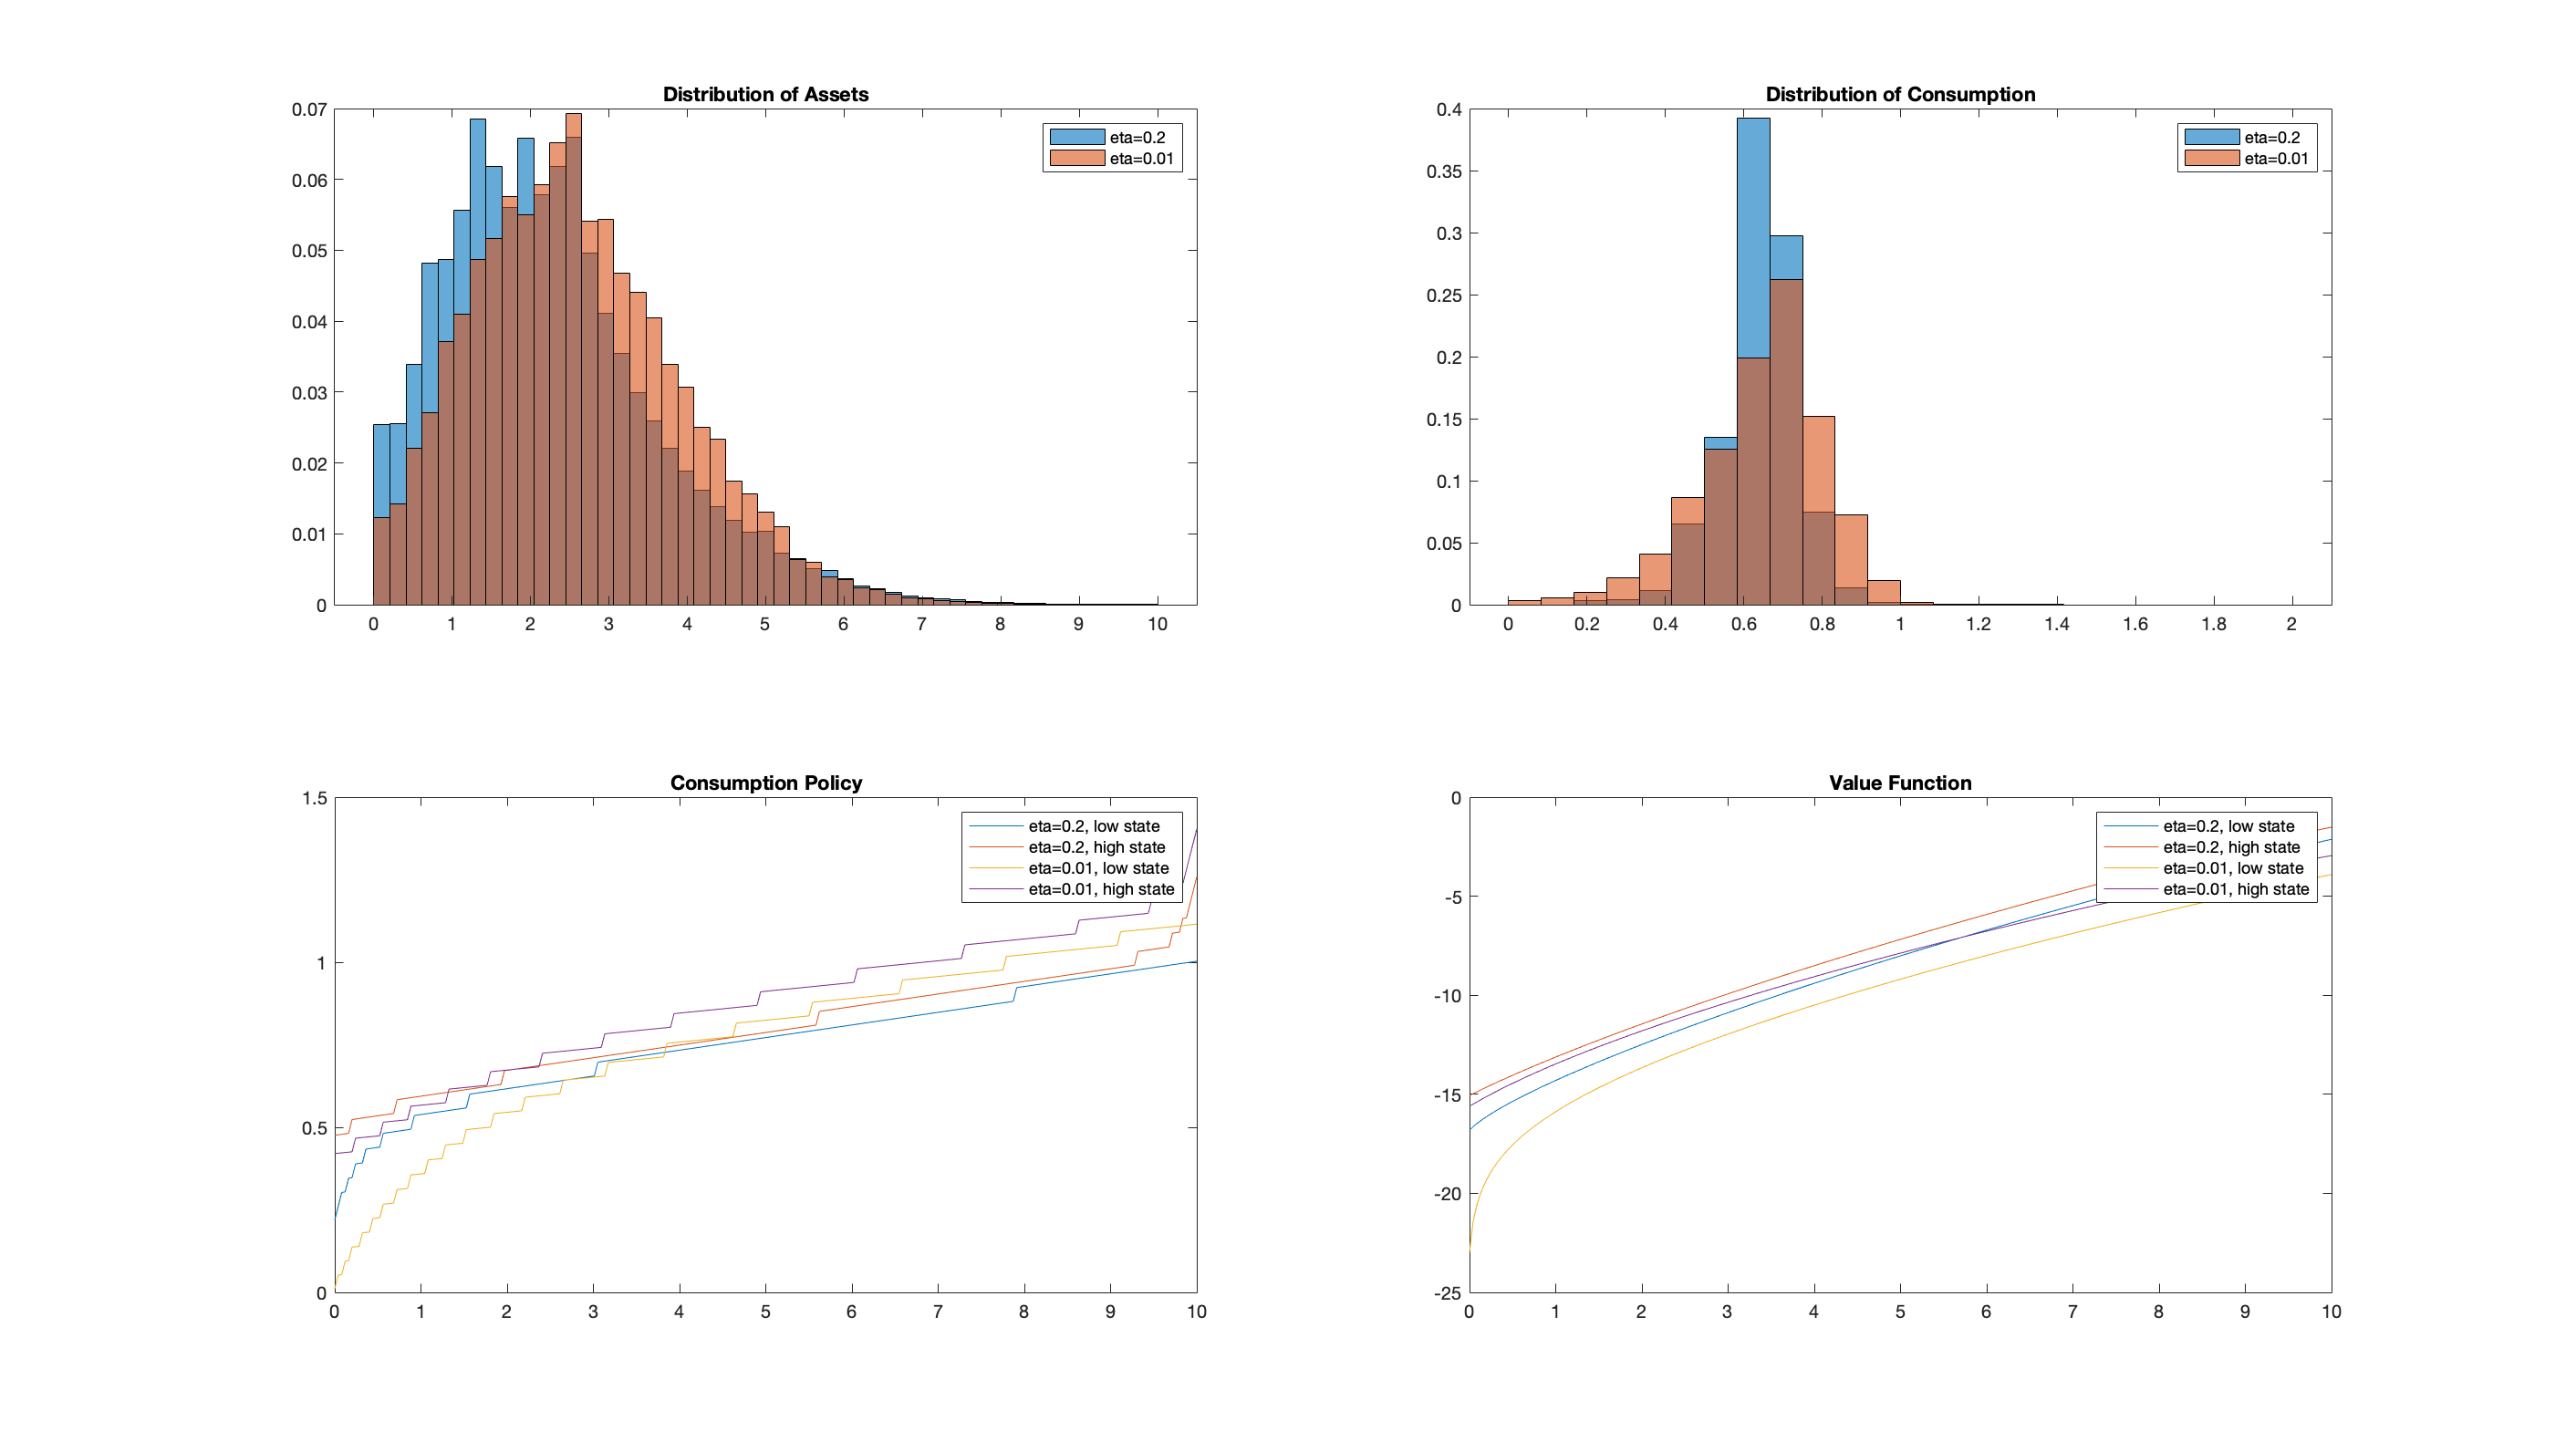
\includegraphics[width=14cm]{ps5fig1}
\end{center}
\end{figure}
\end{document}
	% line of code telling latex that your document is ending. If you leave this out, you'll get an error
